\documentclass[12pt,a4paper]{article}
\usepackage[utf8]{inputenc}
\usepackage{amsmath}
\usepackage{amsfonts}
\usepackage{amssymb}
\usepackage{placeins}
\usepackage{titlesec}

\usepackage{cmap} % для кодировки шрифтов в pdf
\usepackage[T1]{fontenc}
\usepackage{hhline}
\usepackage[unicode]{hyperref}
\usepackage{multirow}
\usepackage{array}
\usepackage{amsmath}
\usepackage{bm}
\usepackage{textcomp}
\usepackage[russian]{babel}
\usepackage{graphicx} % для вставки картинок
\usepackage{amssymb,amsfonts,amsmath,amsthm} % математические дополнения от АМС
\usepackage{indentfirst} % отделять первую строку раздела абзацным отступом тоже
% Поля
\usepackage{geometry}
\geometry{left=2cm}
\geometry{right=1.5cm}
\geometry{top=2.4cm}
\geometry{bottom=2.cm}

%%%%%%%%%%%%%%%%%%%%%%%%%%%%%%%     

\linespread{1.5} % полуторный интервал
\frenchspacing




\begin{document}
	
	\begin{titlepage}
		
		\begin{center}
			\begin{large}
				\textbf{Санкт-Петербургский Политехнический университет\\ Петра Великого\\}
			\end{large}
			\textbf{Институт прикладной математики и механики}\\
			\vspace{0.2cm}
			\textbf{Высшая школа прикладной математики и вычислительной физики}\\
			
		\end{center}
		
		\vspace{3cm}
		\begin{center}
			\textbf{Курсовая работа}\\
			по дисциплине "математическая статистика" \\
			на тему "Анализ пилообразных колебаний излучения плазмы"
		\end{center}
		
		\vspace{3cm}
		
		\vbox{%
			\hfill%
			\vbox{%
				\hbox{Выполнил студент:}%
				\hbox{\break}
				\hbox{ Аникин Александр Алексеевич,}%
				\hbox{группа 3630102$\backslash$80201}%
				\hbox{\break}
				\hbox{\break}
				\hbox{Проверил:}
				\hbox{\break}
				\hbox{к.ф.-м.н., доцент}
				\hbox{Баженов Александр Николаевич}
			}%
		} 
		\vfill
		
		\begin{center}
			Санкт-Петербург, 2021
		\end{center}
		
	\end{titlepage}

	\tableofcontents
	\newpage
	
	\listoffigures
	\newpage

	\section{Постановка задачи}
	
		Даны показания нескольких датчиков, регистрирующих мягкое рентгеновское излучение плазмы в одном эксперименте. В показаниях датчиков иногда наблюдаются пилообразные колебания, предшествующие срыву плазмы. Важно уметь вовремя детектировать такие колебания, чтобы
		предотвращать срыв плазмы. В связи с этим требуется: 
		\begin{itemize}
			\item Представить алгоритм выделения пилообразных колебаний;
			\item Оценить частоту пилообразных колебаний;
		\end{itemize}
	\newpage
	
	\section{Теория}
		\subsection{Пилообразные колебания}
			Пилообразные колебания – периодическое явление в температуре и плотности плазмы, снабжающей топливом термоядерные реакции в токамаках (токамак - тороидальная камера с магнитными катушками) \cite{naked_science}. Пилообразные колебания выглядят как периодический процесс, состоящий в медленном нарастании температуры электронов в центре плазмы, затем на фоне этого нарастания появляются колебания, которые сменяются затем резким сбросом температуры внутри некоторой области. Снаружи от этой области температура резко возрастает. \cite{Kadomcev}
			\FloatBarrier
			\begin{figure}[h!]
				\centering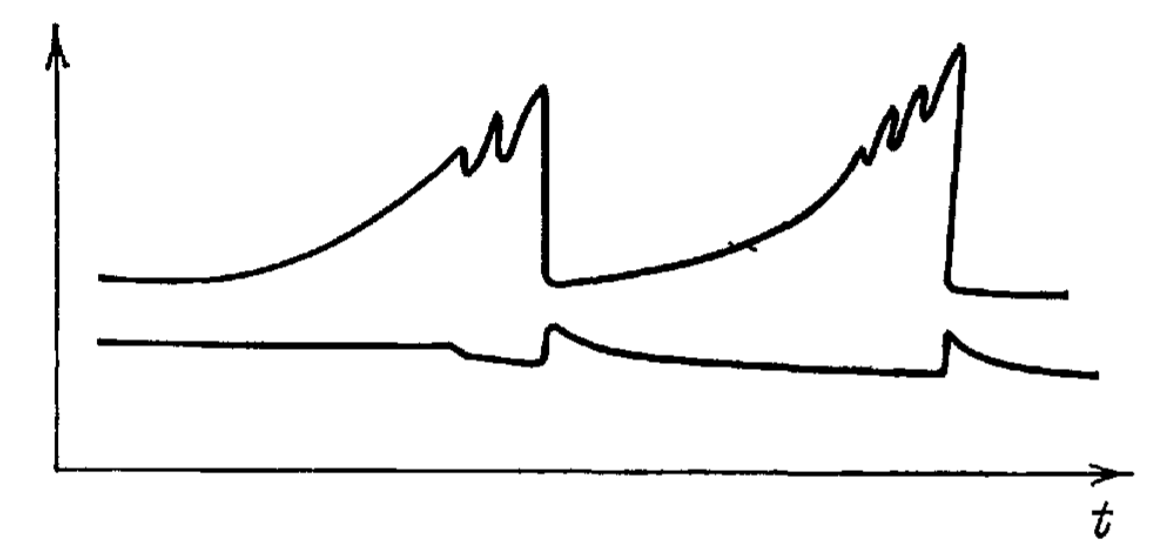
\includegraphics[width=1\linewidth]{./../plots/sawtooth_example.png}
				\caption{Схематическое изображение пилообразных колебаний}
			\end{figure}
			\FloatBarrier
			Было замечено, что явления срывов и пилообразных колебаний схожи, из чего можно рассматривать данный вид колебаний как предпосылку срыва. Этим обуславливается важность изучения данного процесса и детектирования пилообразных колебаний.	
		\subsection{Срыв}
		 Срыв - резкое уплощение плотности тока в шнуре. При срыве из плазмы выбрасывается часть полоидального потока; срыв сопровождается сильными магнитогидродинамическими колебаниями и выбросом заметной доли энергии плазмы на стенки. Большой срыв приводит к полному прекращению тока в плазме. \cite{Kadomcev}
		 
		 \subsection{Частота семплирования}
		 Частота семплирования (или частота дискретизации, англ. sample rate) — частота взятия отсчётов непрерывного по времени сигнала при его дискретизации (в частности, аналого-цифровым преобразователем). Измеряется в герцах. \cite{sample_rate}
		 		 
		 \subsection{Фильтр нижних частот}
		 Фильтр нижних частот (ФНЧ) \cite{lp_filter}:
		 \begin{equation}\label{lp_filter}
		 	y_i=\alpha x_i + (1-\alpha)y_{i-1}, \quad \alpha = \frac{\frac{1}{f_d}}{\frac{1}{2\pi f_c}+\frac{1}{f_d}},
		 \end{equation}
		 где $y_i$ - значение $i$-ого отсчёта выходного сигнала, $x_i$ - значение $i$-ого отсчёта входного сигнала, $f_d$ - частота семплирования ($f_{discretization}$), $f_c$ - частота среза ($f_{cutoff}$).
		 
		 \subsection{Фильтр высоких частот}
		 Фильтр высоких частот (ФВЧ) \cite{hp_filter}:
		 \begin{equation} \label{hp_filter}
		 	y_i=\alpha(y_{i-1}+x_i-x_{i-1}), \quad \alpha = \frac{\frac{1}{2\pi f_c}}{\frac{1}{2\pi f_c}+\frac{1}{f_d}},
		 \end{equation}
		 где $y_i$ - значение $i$-ого отсчёта выходного сигнала, $x_i$ - значение $i$-ого отсчёта входного сигнала, $f_d$ - частота семплирования ($f_{discretization}$), $f_c$ - частота среза ($f_{cutoff}$).
		 
	\newpage
	
	\section{Подготовка данных}
		Данные представлены в бинарном формате в сжатом виде. Декодирование данных производится с помощью Python библиотеки shtRipper \cite{shtRipper}. Далее из декодированных данных извлекаются	временные последовательности показаний датчиков, обработка и вывод которых происходят с помощью языка программирования Python.\\
		Представлен набор данных эксперимента 38515, содержащий 86 сигналов.
		
		\subsection{Первичный анализ данных}
			Первичный анализ данных показал, что:
			\begin{itemize}
				\item Частота семплирования датчиков - 1000 KHz;
				\item Многие из представленных в эксперименте сигналов внешне не содержат как срывов, так и пилообразных колебаний, однако это утверждение было опровергнуто с помощью реализованного алгоритма;
			\end{itemize}
	\newpage
	
	\section{Алгоритм выделения пилообразных колебаний}
		\subsection{Описание алгоритма}
			Предлагается следующий алгоритм для выделения пилообразных колебаний (описан алгоритм выделения для полной последовательности показаний датчика (далее сигнал), но нетрудно проверить, что алгоритм возможно применять для анализа показаний в режиме онлайн). Описание алгоритма с иллюстрациями промежуточных результатов преобразований сигнала на примере данных эксперимента 38515, датчика ФДУК-2 (сигнал с индексом 36):
			
			\FloatBarrier
			\begin{figure}[h!]
				\centering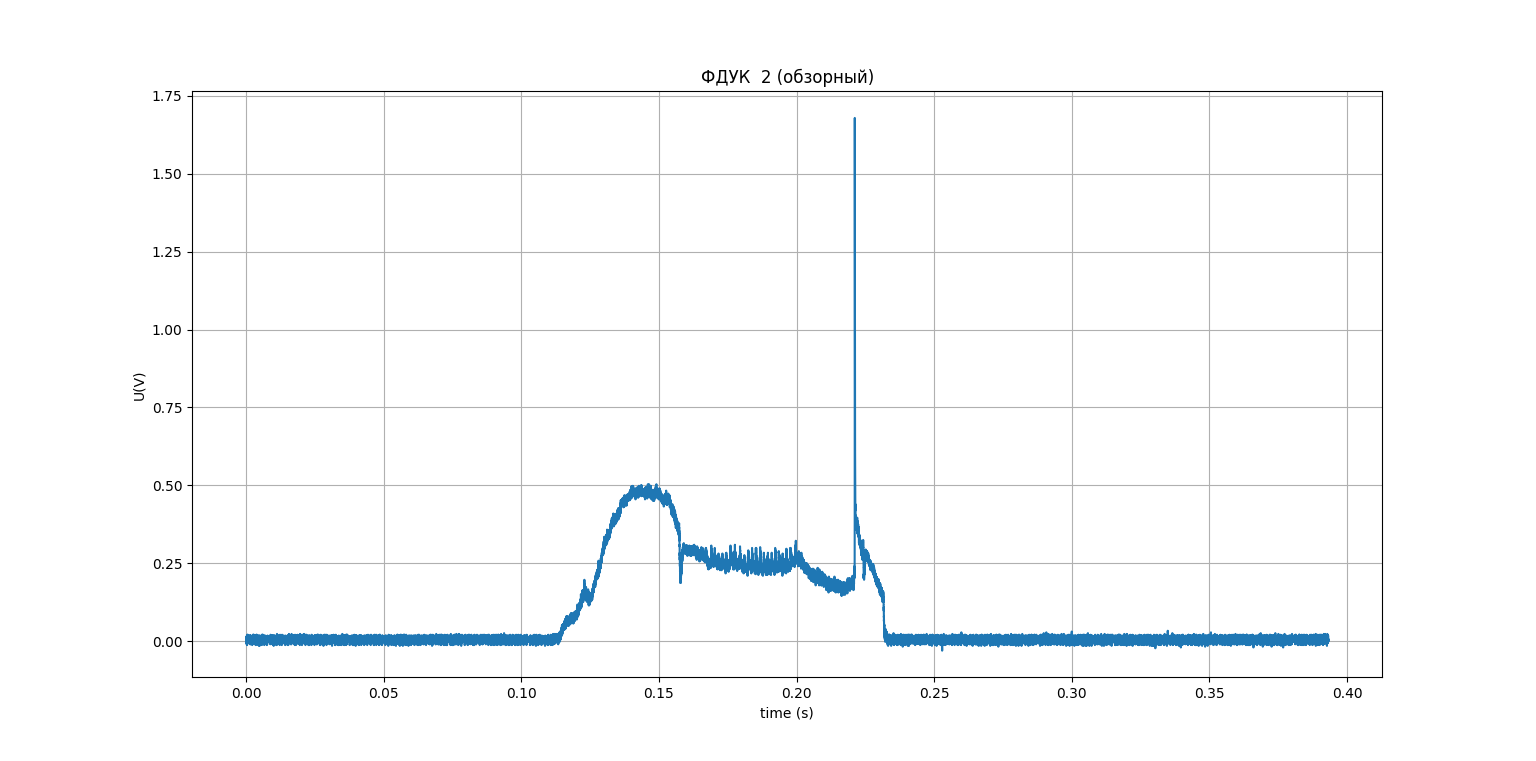
\includegraphics[width=1\linewidth]{./../plots/signal_raw.png}
				\caption{Исходный сигнал}
			\end{figure}
			\FloatBarrier
			
			\begin{enumerate}
				\item Выделяется область для анализа (region of interest, далее ROI). В данном случае ROI - участок сигнала, не являющийся квазистационарным. Таким образом, ROI выделяется путем выделения промежутка со значениями отсчётов, превышающими выборочное среднее.
				\FloatBarrier
				\begin{figure}[h!]
					\centering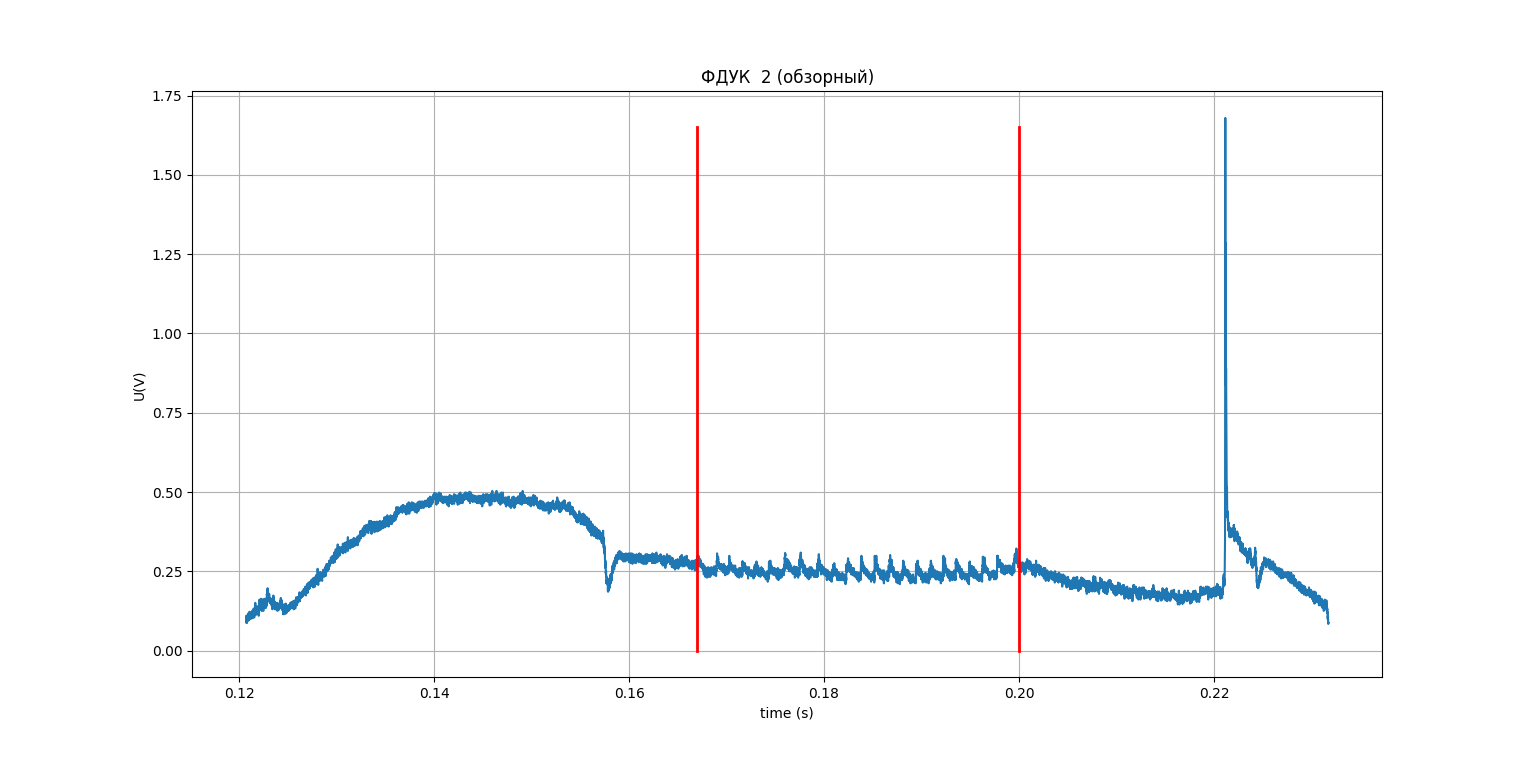
\includegraphics[width=1\linewidth]{./../plots/signal_roi.png}
					\caption{ROI сигнала с выделенной красными линиями областью пилообразных колебаний}
				\end{figure}
				\FloatBarrier
				\FloatBarrier
				\begin{figure}[h!]
					\centering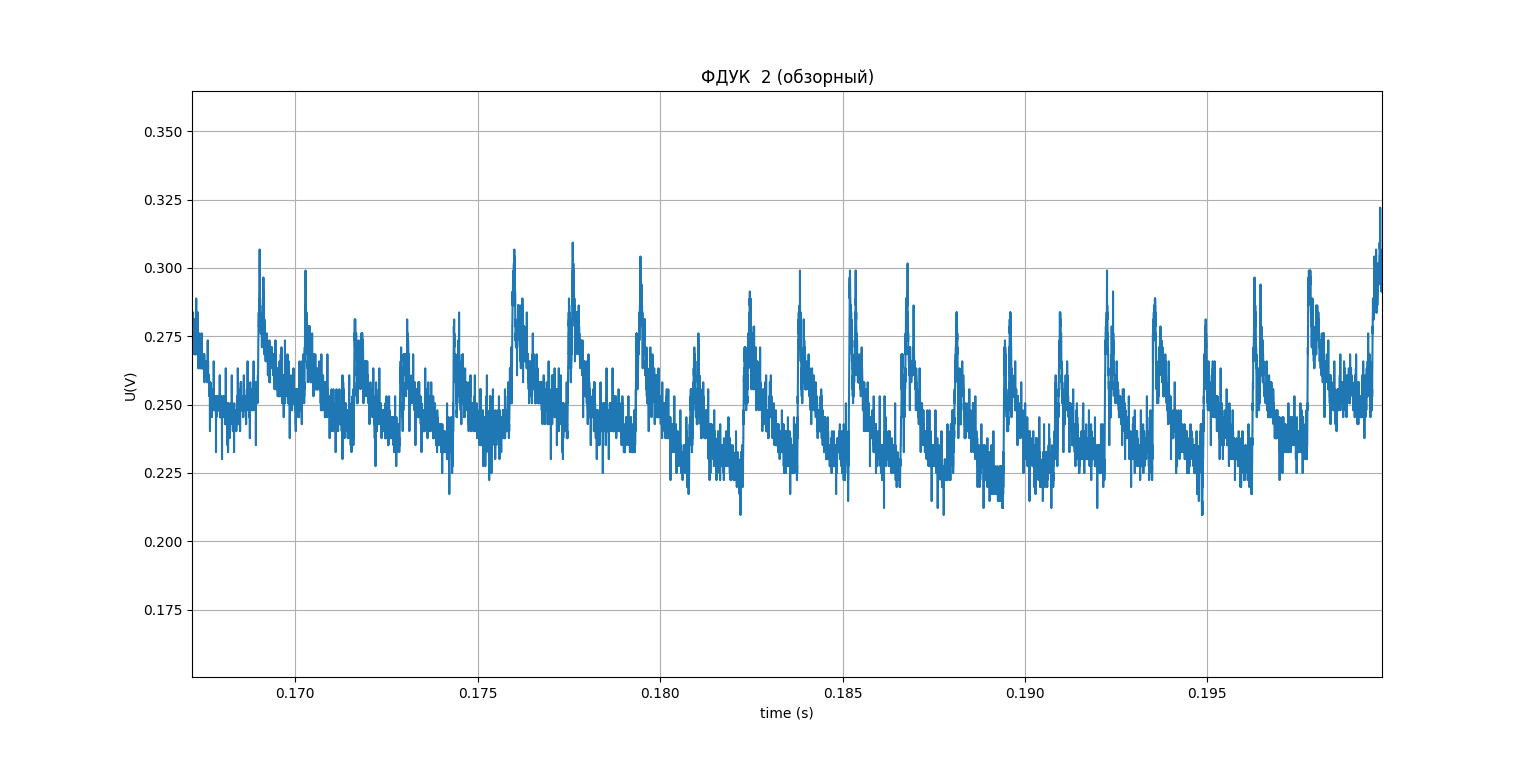
\includegraphics[width=1\linewidth]{./../plots/signal_roi_zoomed.png}
					\caption{участок пилообразных колебаний в приближении}
				\end{figure}
				\FloatBarrier
				
				
				\item Для спрямления исходного сигнала, то есть удаления низкочастотных составляющих применяется ФВЧ (\ref{hp_filter}).
				\FloatBarrier
				\begin{figure}[h!]
					\centering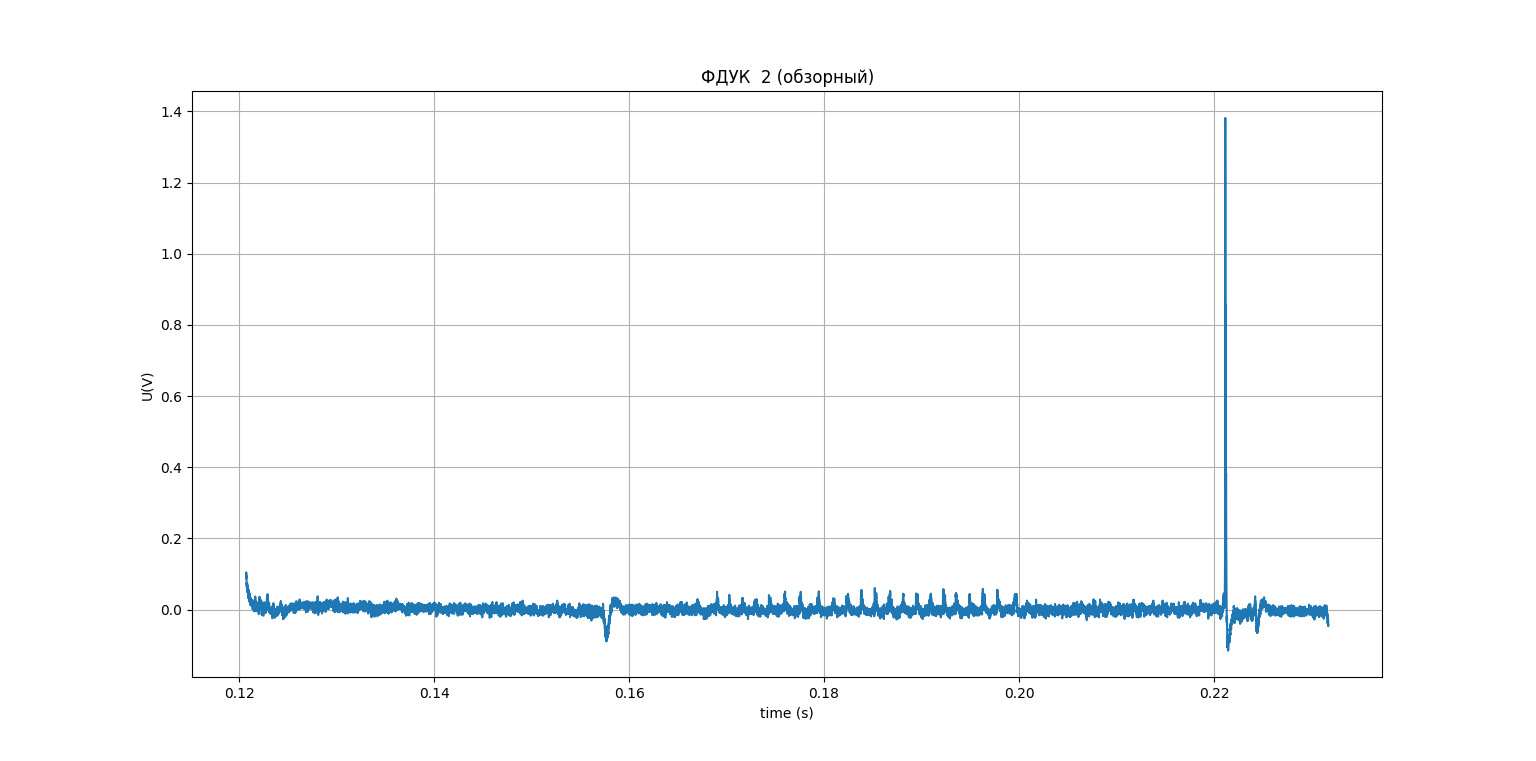
\includegraphics[width=1\linewidth]{./../plots/signal_hp_filtered.png}
					\caption{Спрямлённый сигнал после применения ФВЧ}
				\end{figure}
				\FloatBarrier
				
				\item Находится первая производная спрямленного сигнала путем применения сглаживающего цифрового дифференцирующего фильтра (ЦДФ) \cite{DDF} по следующей формуле:
					\begin{equation}\label{DDF}
						y(n) = \sum_{k=1}^{M}\frac{1}{M(M+1)}\Delta_k, \quad \Delta_k = x(n+k) - x(n-k),
					\end{equation}
					где $M \geq 2$ - порядок фильтра, $x(n)$ - значение $n$-ого отсчёта входного сигнала, $y(n)$ - значение $n$-ого отсчёта выходного сигнала.
				\FloatBarrier
				\begin{figure}[h!]
					\centering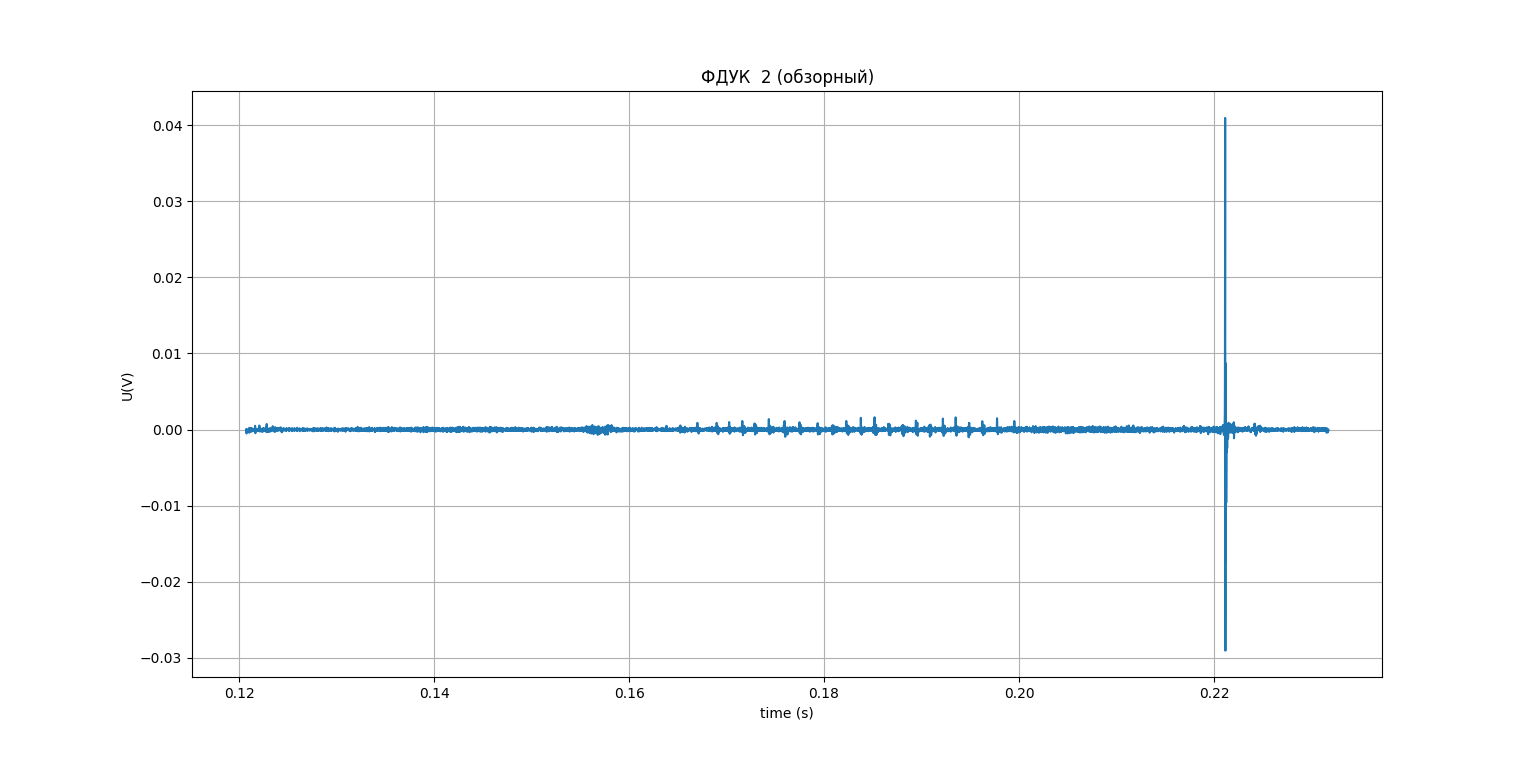
\includegraphics[width=1\linewidth]{./../plots/signal_1st_der.png}
					\caption{Первая производная сигнала, вычисленная с помощью ЦДФ (\ref{DDF})}
				\end{figure}
				\FloatBarrier
				
				\item Берется модуль от первой производной спрямленного сигнала.
				\FloatBarrier
				\begin{figure}[h!]
					\centering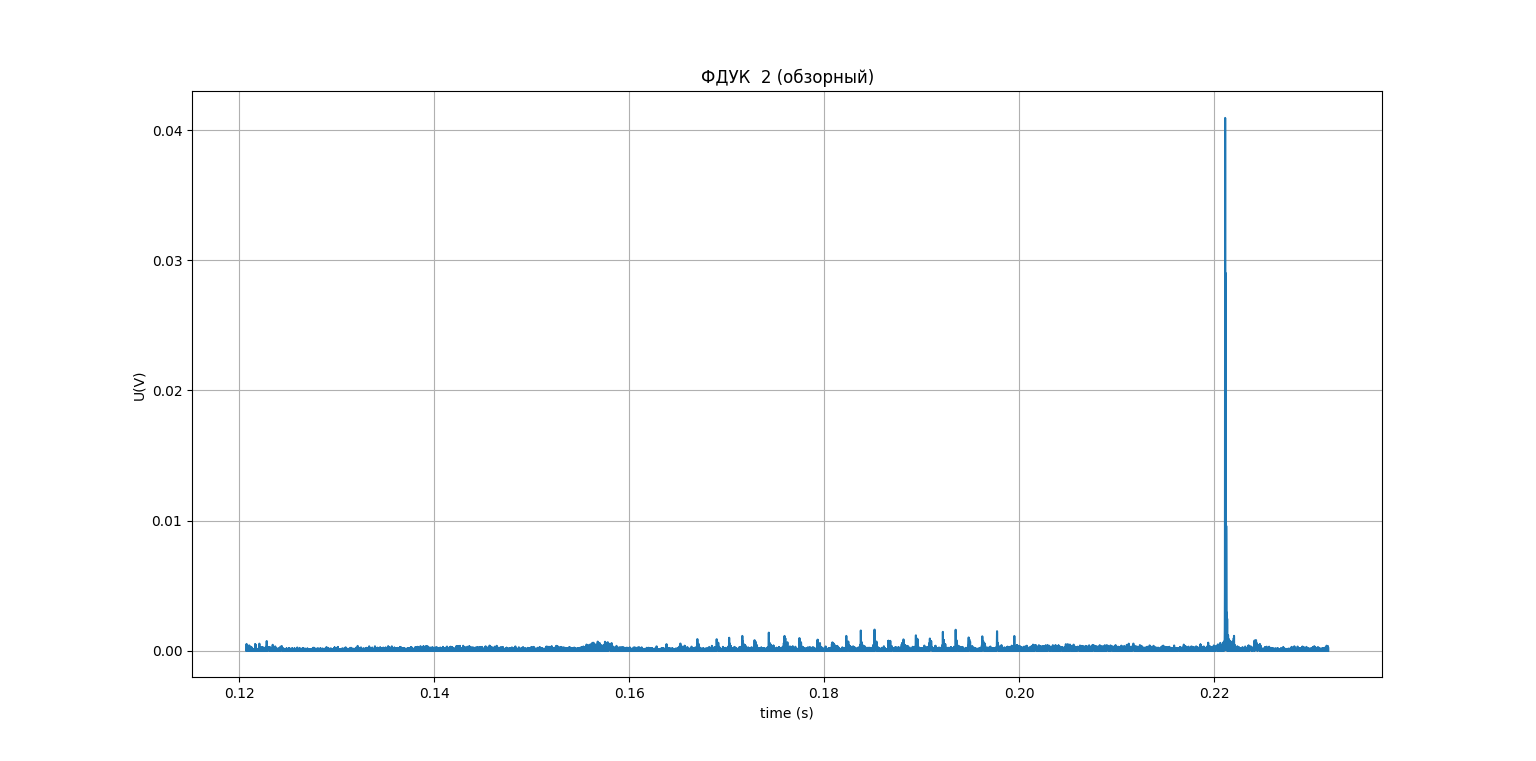
\includegraphics[width=1\linewidth]{./../plots/signal_1st_der_abs.png}
					\caption{Модуль первой производной}
				\end{figure}
				\FloatBarrier
				
				\item Применяется ФНЧ (\ref{lp_filter}) для удаления высокочастотного шума.
				\FloatBarrier
				\begin{figure}[h!]
					\centering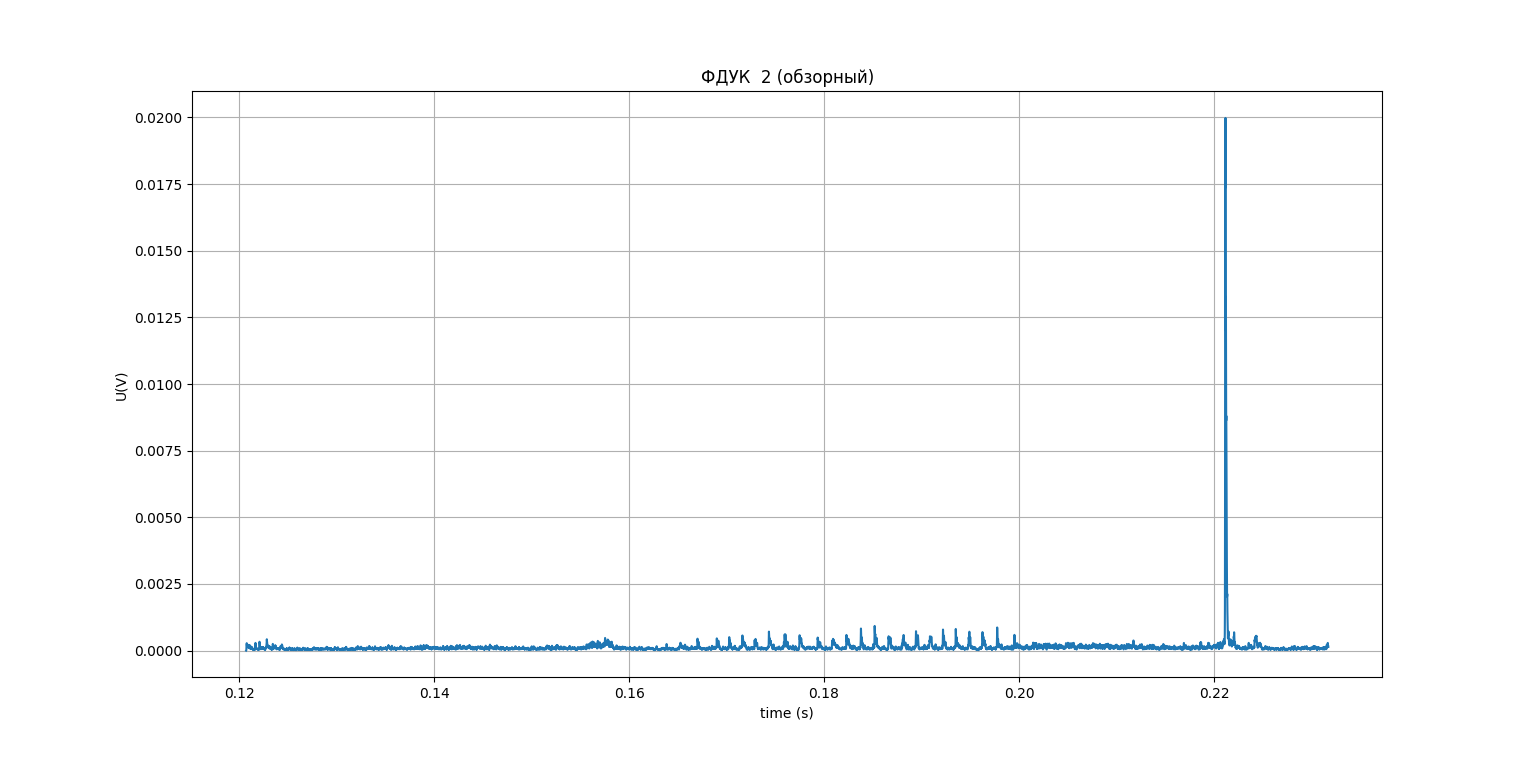
\includegraphics[width=1\linewidth]{./../plots/signal_lp_filtered.png}
					\caption{Спрямлённый сигнал после применения ФНЧ}
				\end{figure}
				\FloatBarrier
				
				\FloatBarrier
				\begin{figure}[h!]
					\centering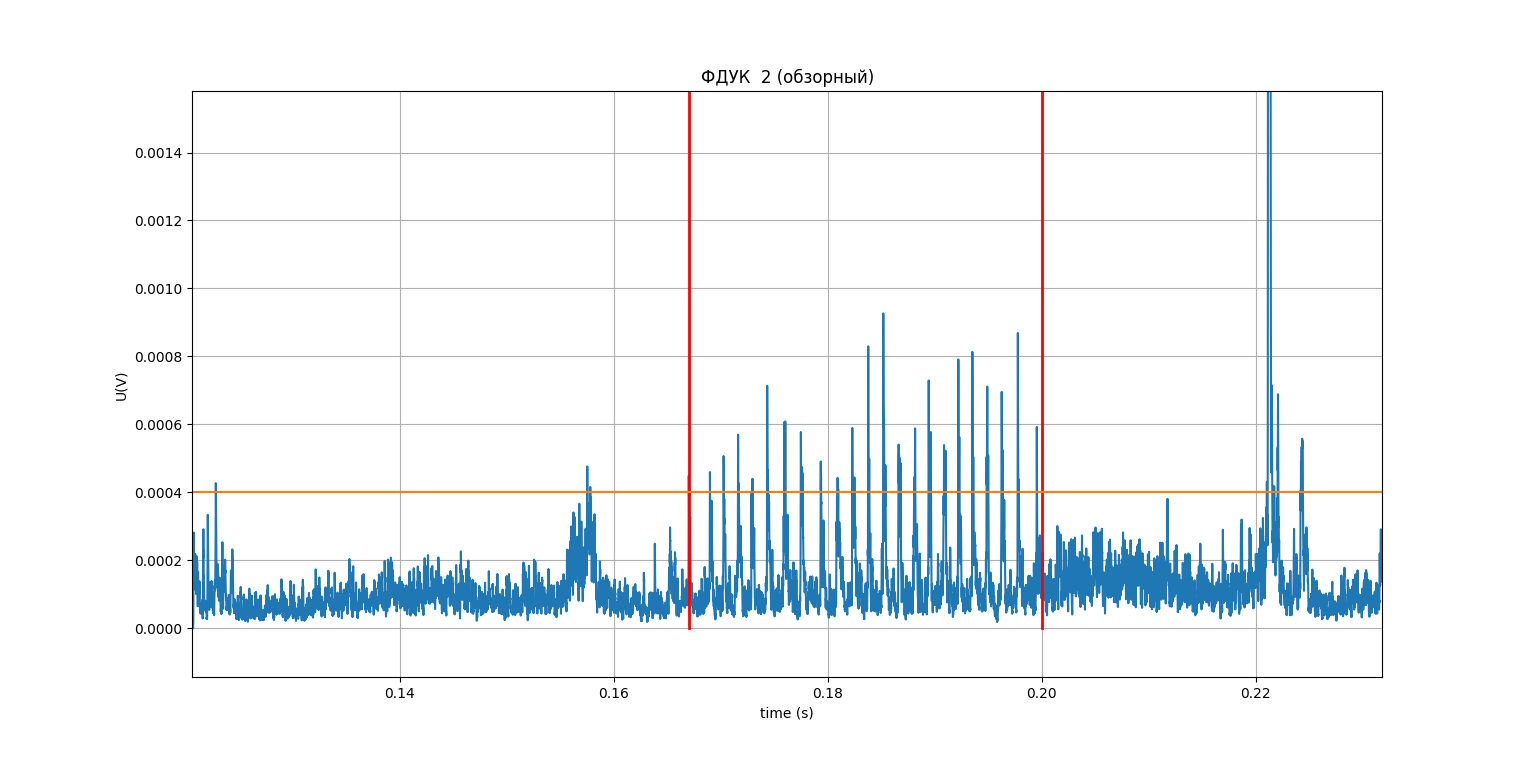
\includegraphics[width=1\linewidth]{./../plots/signal_lp_filtered_zoomed_v2.png}
					\caption{Спрямлённый сигнал после применения ФНЧ с выделенной областью пилообразных колебаний в приближении}
				\end{figure}
				\FloatBarrier
				
				\item Индикатором пилообразных колебаний будет служить наличие и частота появления значений	сигнала выше некоторого порога (в данном случае 0.0004).
			\end{enumerate}
			
			Предложенный алгоритм позволяет достаточно точно определять участок	с пилообразными колебаниями в сигнале датчика: большая часть значений выше порога действительно принадлежит искомому участку. Также стоит отметить, что алгоритм без проблем можно применять (после некоторой переработки шагов, в которых применяются фильтры) в реальном времени, так как он не требует для работы всей последовательности наблюдений.	В целом алгоритм хорошо показал себя на данном сигнале. Подобный алгоритм также описан в работе \cite{Algoritm}, и судя по всему, успешно применяется на практике.
		
		\subsection{Параметры алгоритма}
			Алгоритм параметризуется следующими величинами:
			\begin{itemize}
				\item Порядком ЦДФ
				\item Пороговым значением
			\end{itemize}
		
			Стоит отметить, что параметры ФВЧ на шаге №2 и ФНЧ на шаге №5 также могут зависеть от условий эксперимента, однако такой зависимости не наблюдалось при обработке предоставленных данных. Можно предложить альтернативу последнему шагу, которая не требует задания порогового значения, повышая таким образом устойчивость алгоритма. Такая альтернатива - оценка плотности распределения локальных максимумов в некотором окне: во время пилообразных колебаний плотность понижается.
			
			\FloatBarrier
			\begin{figure}[h!]
				\centering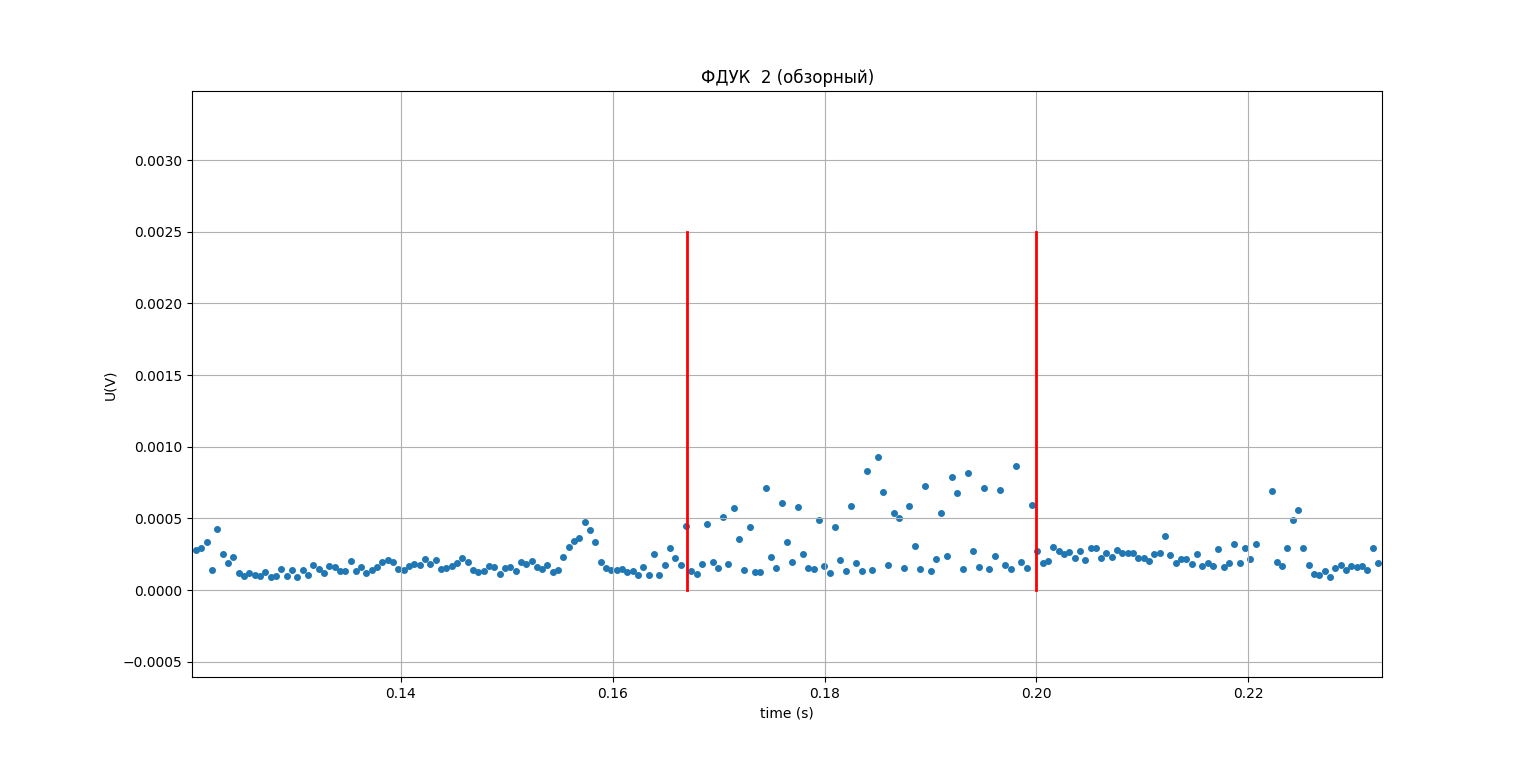
\includegraphics[width=1\linewidth]{./../plots/sawtooth_alternative_detection.png}
				\caption{Локальные максимумы итогового сигнала в окне размера 500 (0.0005 сек)}
			\end{figure}
			\FloatBarrier	
		\newpage
		
		\section{Оценка частоты пилообразных колебаний}
		После выделения участка пилообразных колебаний можно попробовать оценить их частоту, а точнее ее эволюцию. Для решения подобных задач широко применяются два способа: преобразование Фурье и анализ автокорреляционной функции. 
		\begin{itemize}
			\item Применение первого способа к имеющимся данным затруднительно, так как интересующие нас частоты лежат в полосе от 0 до 1 KHz, в то время как переход из временной области в частотную
			с помощью преобразования Фурье дает нам спектр от 0 до 500 KHz Кроме того, сигнал сильно зашумлен, поэтому даже после применения ФНЧ и ФВЧ выделить собственные частоты пилообразных колебаний не представляется возможным без априорных знаний об искомой полосе частот.
			
			\item Второй способ мог бы решить задачу, однако его экстраполяция на случай с переменной частотой, вообще говоря, нетривиальна.
		\end{itemize}
		
		Для решения задачи с учетом специфики предоставленных данных предлагается следующий алгоритм на примере данных эксперимента 38515, датчика ФДУК-2 (сигнал с индексом 36):
		
		\FloatBarrier
		\begin{figure}[h!]
			\centering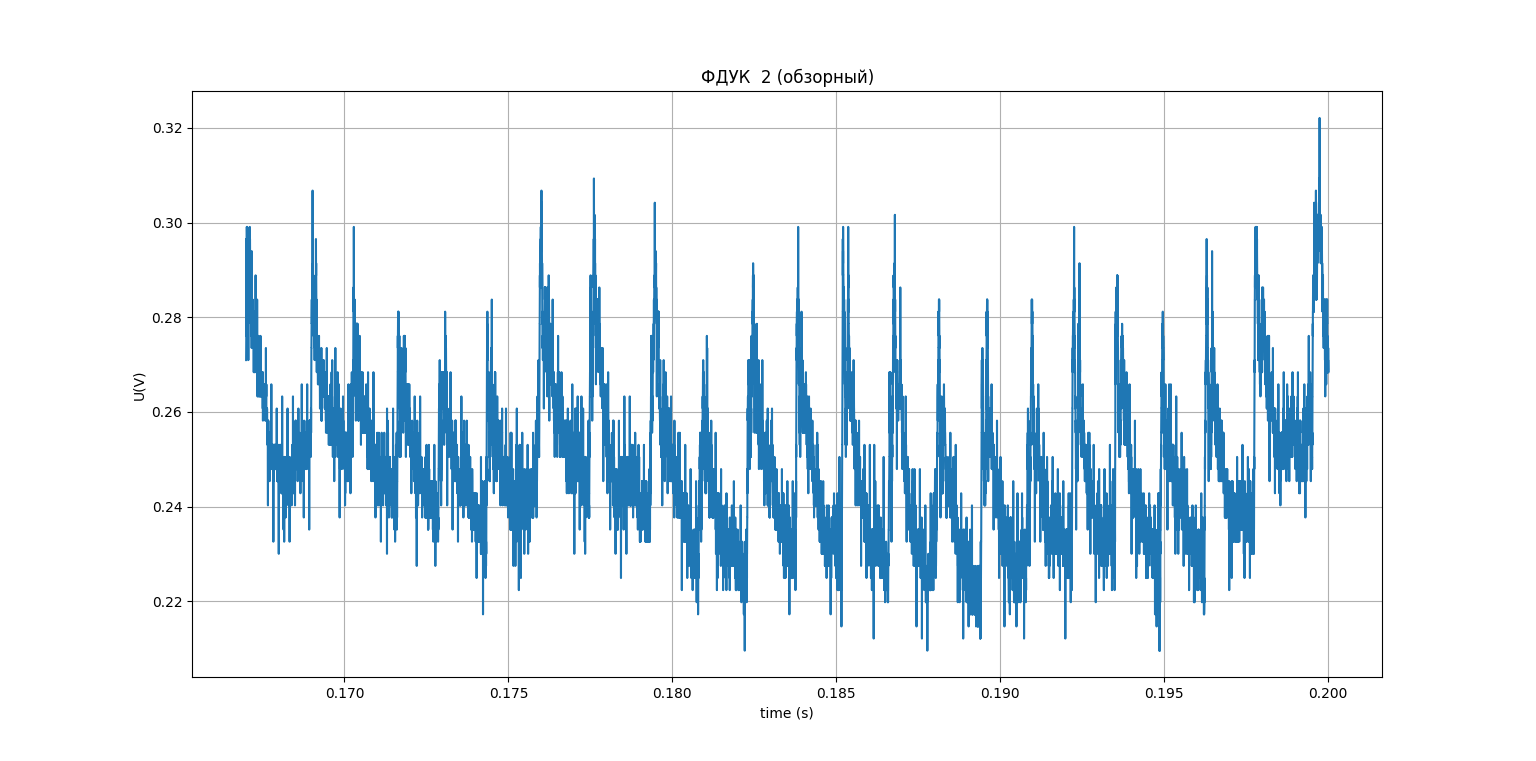
\includegraphics[width=1\linewidth]{./../plots/freq_raw.png}
			\caption{Исследуемый участок пилообразных колебаний}
		\end{figure}
		\FloatBarrier
		
		\begin{enumerate}
			\item Спрямляется участок, содержащий пилообразные колебания с помощью ФВЧ с частотой среза
			250 Гц.
			
			\FloatBarrier
			\begin{figure}[h!]
				\centering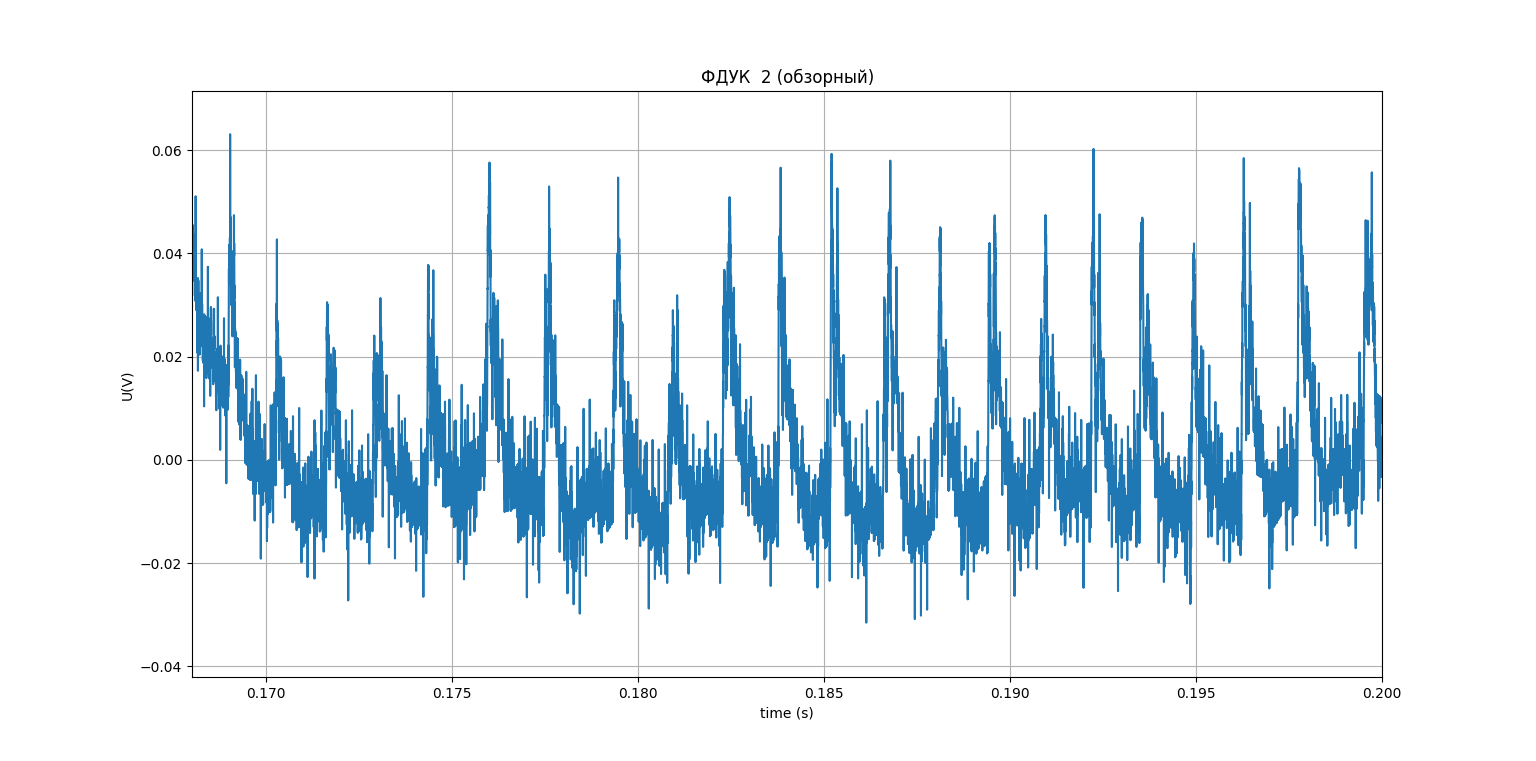
\includegraphics[width=1\linewidth]{./../plots/freq_hp_filtered.png}
				\caption{Спрямленный участок пилообразных колебаний после применения ФВЧ}
			\end{figure}
			\FloatBarrier
			
			\item Удаляется высокочастотные шумы спрямленного сигнала с помощью ФНЧ с частотой среза 200
			Гц.
		
			\item Выделяются все точки пересечения сигнала с осью абсцисс.
			\FloatBarrier
			\begin{figure}[h!]
				\centering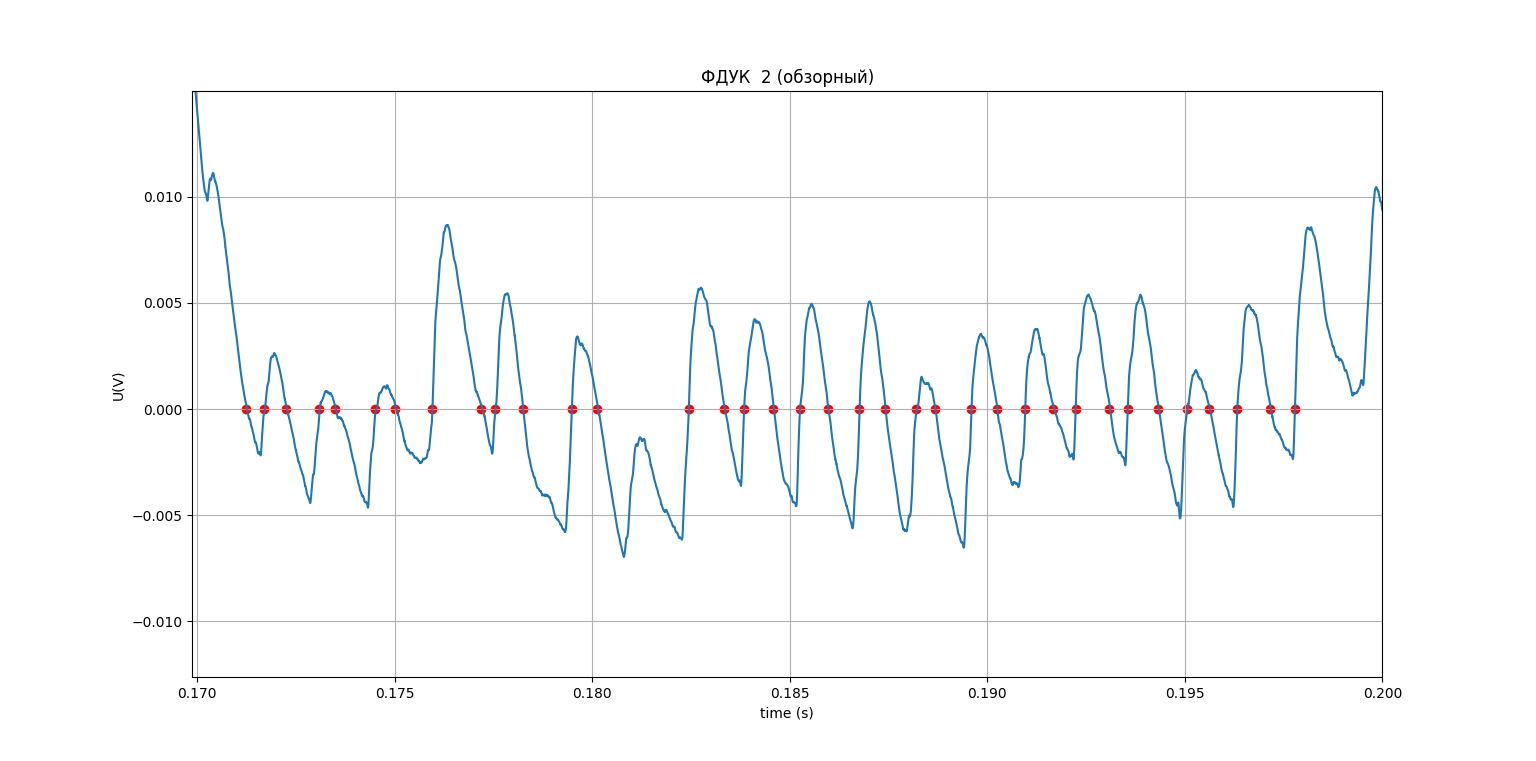
\includegraphics[width=1\linewidth]{./../plots/freq_lp_filtered.png}
				\caption{Участок пилообразных колебаний после применения ФНЧ с отмеченными пересечениями с осью абциcс}
			\end{figure}
			\FloatBarrier
			
			\item Вычитаются полученные значения друг из друга через одного, получаются мгновенные периоды
			колебаний.
			
			\item Из периодов получаются мгновенные частоты, то есть функцию частоты от времени.
			
			\item Для сглаживания полученной функции применяем любой сглаживающий фильтр, например,
			фильтр Баттерворта \cite{butter}.
			\FloatBarrier
			\begin{figure}[h!]
				\centering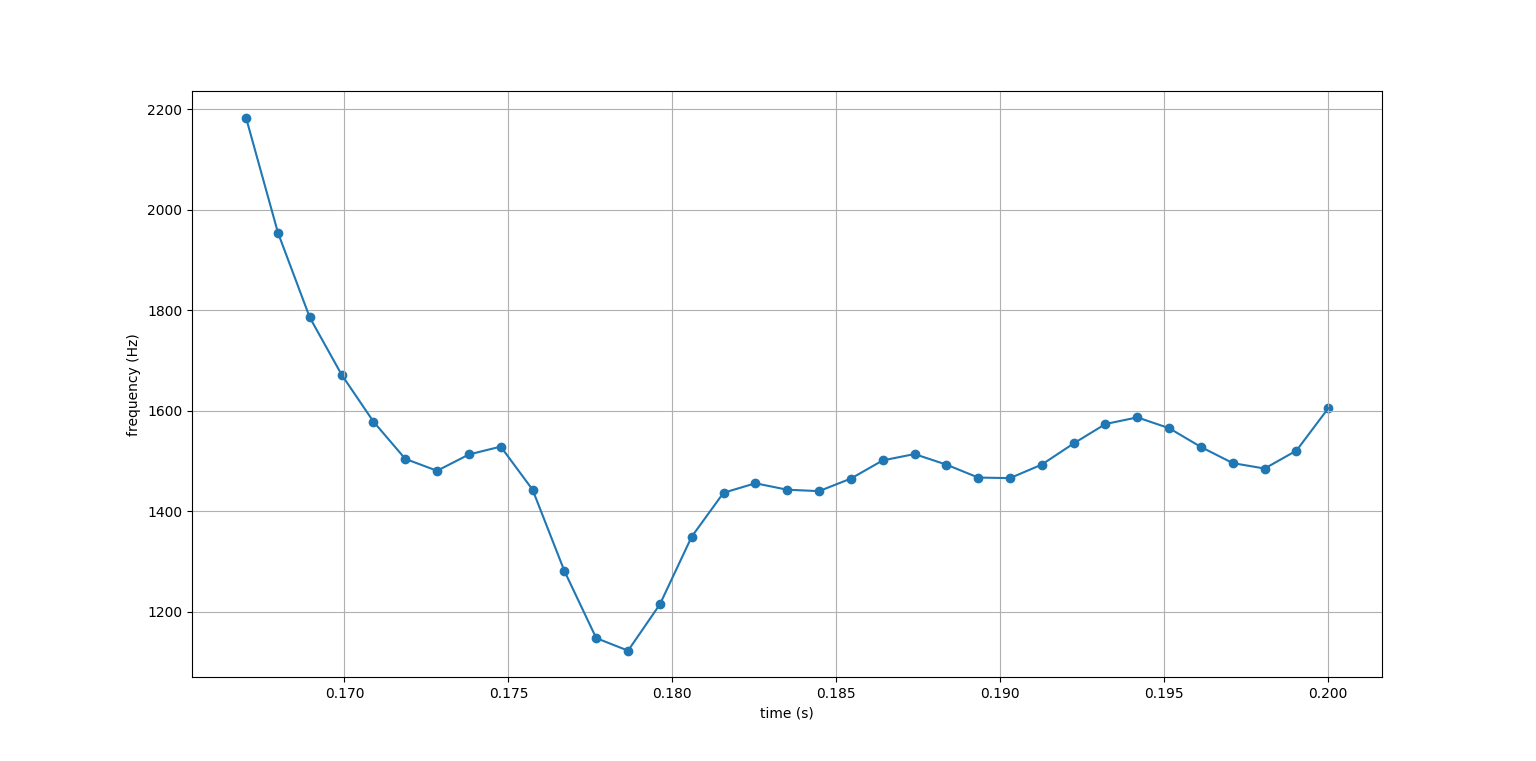
\includegraphics[width=1\linewidth]{./../plots/freq_plot.png}
				\caption{Итоговая функция частоты от времени}
			\end{figure}
			\FloatBarrier
			
			
		\end{enumerate}
	\newpage
	
	\section{Выводы}
	В данной работе были описаны, реализованы и проиллюстрированы алгоритмы выделения пилообразных колебаний в сигнале и анализа их частоты. Реализация производилась при помощи языка Python с подключаемыми пакетами Matplotlib, Numpy, SciPy и сторонней библиотеки shtRipper.\\
	
	Алгоритм выделения участка пилообразных колебаний с производит вычисления приемлемой точностью. К его достоинствам относятся:
	\begin{itemize}
		\item Возможность использования одновременно со съемом данных;
		\item Гибкость выбора критерия детекции;
	\end{itemize}
	Из недостатков можно выделить:
	 \begin{itemize}
		\item Необходимость параметризации порядком ЦДФ и пороговым значением отсчётов участка пилообразных колебаний (однако, существует альтернативный критерий выделения, который не требует параметризации, но может оказаться недостаточно точным при наличии большого количества выбросов);
	 \end{itemize}
 	
 	Алгоритм выделения частот пилообразных колебаний также демонстрирует приемлемую точность, однако вопрос удовлетворительного способа и коэффициента сглаживания требует рассмотрения.
 	
 	\newpage
 	\begin{flushleft}
		\begin{thebibliography}{1}
			\addcontentsline{toc}{section}{\bibname}
			
			\bibitem{shtRipper} Библиотека shtRipper. URL: \url{https://gitlab.spectraltech.ru/Rezenter/shtRipper}

			\bibitem{Kadomcev} Кадомцев В.В. Перезамыкание силовых линий. УФН. - Москва: Физический институт им П. Н. Лебедева РАН, 1987. 27с.
						
			\bibitem{naked_science} Пилообразные колебания.  URL: \url{https://naked-science.ru/article/sci/otkryt-mehanizm-stabilizacii}
			
			\bibitem{butter} Фильтр Баттерворта. URL: \url{https://docs.scipy.org/doc/scipy/reference/generated/scipy.signal.butter.html}

			\bibitem{hp_filter} Фильтр высоких частот. URL: \url{https://en.wikipedia.org/wiki/High-pass_filter}

			\bibitem{lp_filter} Фильтр нижних частот. URL: \url{https://en.wikipedia.org/wiki/Low-pass_filter}
						
			\bibitem{sample_rate} Частота семплирования. URL: \url{https://en.wikipedia.org/wiki/Sampling_(signal_processing)#Sampling_rate}
			
			\bibitem{Algoritm} Felici, F. and Le, H.B. and Paley, J.I. and Duval, B. and Coda, S. and Moret, J.M and Bortolon, Alessandro and Federspiel, Lucia and Goodman, T. and Hommen, Gillis and Karpushov, Alexander and Piras, F. and Pitzschke, Andreas and Romero, Je sus and Sevillano, M. and Sauter, O. and Vijvers, Wouter. Development of real-time plasma analysis and control algorithms for the TCV tokamak using SIMULINK. Fusion Engineering and Design, vol. 89, issue 3, 2014, pp. 165-176
			
			\bibitem{DDF} S. Usui, I. Amidror. Digital Low-Pass Differentiation for Biological Signal Processing. IEEE Transactions on Biomedical Engineering, vol. BME-29, issue 10, 1982, pp. 686-693
			
			
						
			\end{thebibliography}
	\end{flushleft}

\end{document}